
\section{Combining Forces\footnote{
1990-93 Dept. of Physics and Astronomy, Dickinson College. Supported by FIPSE
(U.S. Dept. of Ed.) and NSF. Portions of this material may have been modified
locally and may not have been classroom tested at Dickinson College.
}}

\makelabheader %(Space for student name, etc., defined in master.tex or labmanual_formatting_commands.tex)

\textbf{Objectives}

\begin{itemize}
\item To understand how different forces can act together to make up a combined force.~ 
\item To establish a definition of combined force as that which changes the motion
of an object.
\item To understand the motion of an object with no force applied to it and how Newton's
First Law describes this motion.
\end{itemize}
\textbf{Overview}

In this unit, you will explore what happens when more than one force is applied
to an object. Also, you will be asked to consider the special case when the
object moves with a constant velocity, so that the object's acceleration is
zero. What combination of forces must be applied to an object to keep it moving
with a constant velocity when there is almost no friction? You can answer this
question by collecting force and motion data again with the force probe and
motion detector. The answer to this question will lead you to the discovery
of Newton's First Law (in a situation where friction can be neglected).

\textbf{Apparatus}

\begin{itemize}
\item Force probe
\item Motion detector
\item Dynamics cart (with flag) and track
\item Low friction pulleys (2) and string
\item Variety of hanging masses
\item Pasco 550 Interface
\item Capstone software (\filename{V\_A\_F\_Graphs.cap} experiment file)
\end{itemize}
\textbf{Net Force: Combining Applied Forces }

As you know, vectors are mathematical entities with both magnitude and
direction. Thus a one-dimensional vector can have a direction along the positive
x-axis or along the negative x-axis. Vectors pointing in the same direction
add together and vectors pointing in opposite directions subtract from each
other. Quantities which have vector behavior are often denoted by a letter with
a little arrow above it or by a boldface letter (i.e., \textbf{F}). The sum of
several vectors is often denoted by placing a summation sign in front of a vector
symbol (i.e., \( \sum {\bf F}  \)). In the next two activities you will
investigate how combined forces change the motion of an object.

\textbf{Activity 1: Two Forces in the Same Direction}

(a) Suppose you apply two 0.5-N forces to the cart in the same direction. How
will the motion compare with the motion you observed in the previous unit for
a 1-N force?
\answerspace{20mm}

\pagebreak[3]
(b) Test your predictions. Set up a second pulley next to the first one, attach
a second string from the force probe hook over the second pulley, and hang 50
g from each string. Graph the motion as in the previous unit. Repeat until you
get a good run and sketch the results on the axes below. Don't forget to label
the axes.

%\vspace{0.3cm}
%{\par\centering 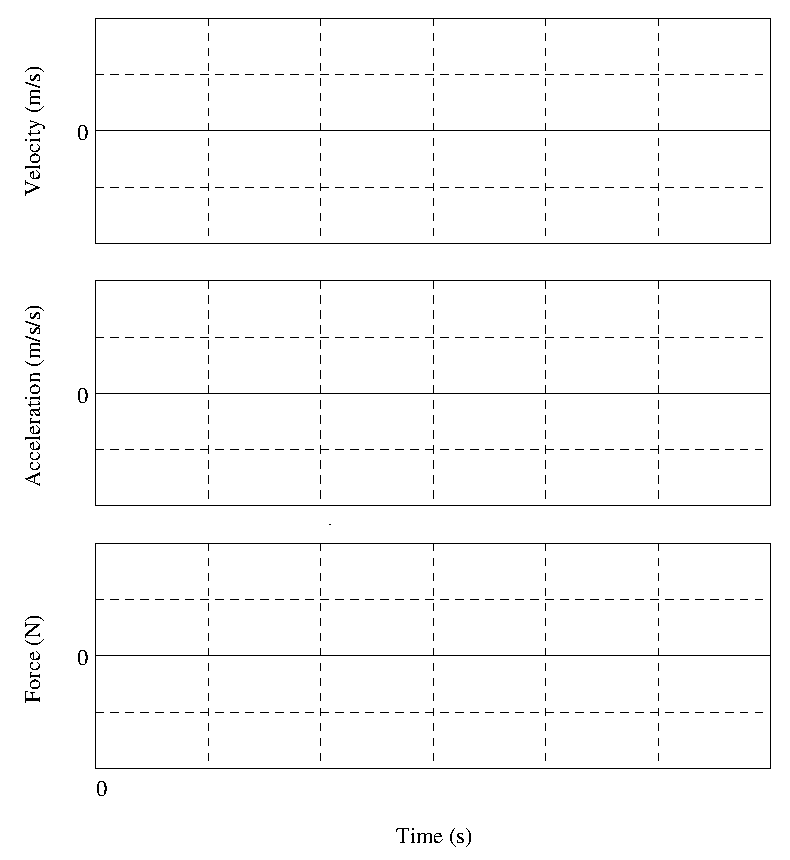
\includegraphics{force2/force2_fig4.eps} \par}
%\vspace{0.3cm}
\begin{lab_groupplot}*{}[lab_grid,
	group style={
		group size=1 by 3,
		xlabels at=edge bottom,
		vertical sep=0.3in,
		},
	width=4.2in,  height=1.4in,
	xlabel=Time (s),
	xmin=0, xmax=12,
	xtick distance = 2, 
	ytick distance = 1, 
	minor tick num=1,
	ytick = {-1,0,1},
	yticklabels = {$-$, 0, $+$},
	]
\nextgroupplot[
	ymin=-1,ymax=1, 
	ylabel={Velocity (m/s)},
	]
\nextgroupplot[
	ymin=-1,ymax=1, 
	ylabel={Acceleration (m/s$^2$)},
	]
\nextgroupplot[
	ymin=-1,ymax=1, 
	ylabel={Force (N)},
	]
\end{lab_groupplot}

(c) Do the results agree with your predictions? Explain.
\answerspace{30mm}

(d) Draw arrows in the space below that represent a scale drawing of the magnitudes
and directions of the forces applied to the cart in this activity and the previous
one.
\answerspace{30mm}

\pagebreak[3]
\textbf{Activity 2: Two Equal Forces in Opposite Directions}

(a) Suppose two equal and opposite forces were applied to the cart. What would
be the resulting motion?
\answerspace{10mm}

\pagebreak[2]
(b) Test your predictions. Move one of the pulleys to the other end of the table
and hang 100 g from each string. Release the cart. Does the resulting motion
agree with your predictions? Explain.
\answerspace{20mm}

(c) Draw a force diagram to scale below.
\answerspace{20mm}

\textbf{Activity 3: Two Unequal Forces in Opposite Directions}

(a) Suppose you hang 150 g from the string above the motion detector and 50
g from the string at the other end of the table. What will be the resulting
motion and how will it compare with the motions observed in Activities 1 and
2?
\answerspace{20mm}

(b) Test your predictions by graphing the motion. Repeat until you get a good
run and sketch your results as dashed lines on the axes in Activity 2.

(c) Do the results agree with your predictions? Explain.
\answerspace{20mm}

(d) Draw a force diagram (to scale) for this situation in the space below.
\vspace{10mm}

(e) Do one-dimensional forces seem to behave like one-dimensional vectors? Why
or why not?
\answerspace{20mm}

(f) When more than one force is acting on an object, what is it that determines
the acceleration of the object?
\answerspace{20mm}

\pagebreak[2]
\textbf{Activity 4: Motion at a Constant Velocity}

(a) Suppose the cart is moving with the velocity which is shown on the velocity-time
graph below. Sketch on the axes below the acceleration-time graph of the cart,
and the force-time graph of the combined force after the cart begins moving.

%\vspace{0.3cm}
%{\par\centering 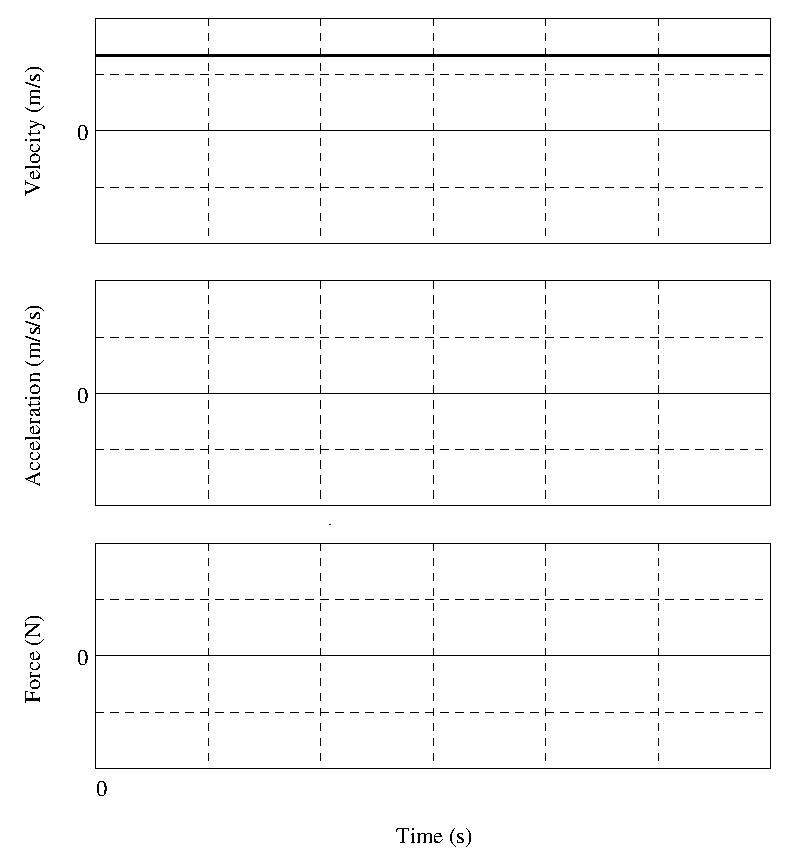
\includegraphics{combining/combining_fig1.eps} \par}
%\vspace{0.3cm}
\begin{lab_groupplot}*{}[lab_noticks_2quads,
	group style={group size=1 by 3},
	width=2.5in,  height=1.4in,
	plus_minus_zero_labels,
	xlabel=Time,
	]
\nextgroupplot[ylabel=Velocity,]
	\addplot {0.6};
\nextgroupplot[ylabel=Acceleration,]
\nextgroupplot[ylabel=Force,]
\end{lab_groupplot}

(b) Describe in words the acceleration of the cart and the combined force needed
to keep it moving at a constant velocity.
\answerspace{15mm}

(c) Test your prediction. Remove the strings from the force probe and give the
cart a push away from the motion detector. Notice that the cart slows down and
eventually stops. This is due to the small amount of friction that exists. Replace
one of the strings and hang a small mass from the string over the pulley at
the far end of the table to balance the frictional force. Push the cart to see
if it moves with approximately constant velocity. Adjust the hanging mass such
that the cart moves with approximately constant velocity. Then graph the motion
of the cart, using the file \filename{V\_A\_F\_Graphs.cap}. Repeat until you get a good run and sketch the results on the axes
below. Don't forget to label the time scale on the axes. If your hand was still
in contact with the cart after the graphing started, indicate with an arrow
the time when the push stopped.

\pagebreak[2]
%\vspace{0.3cm}
%{\par\centering 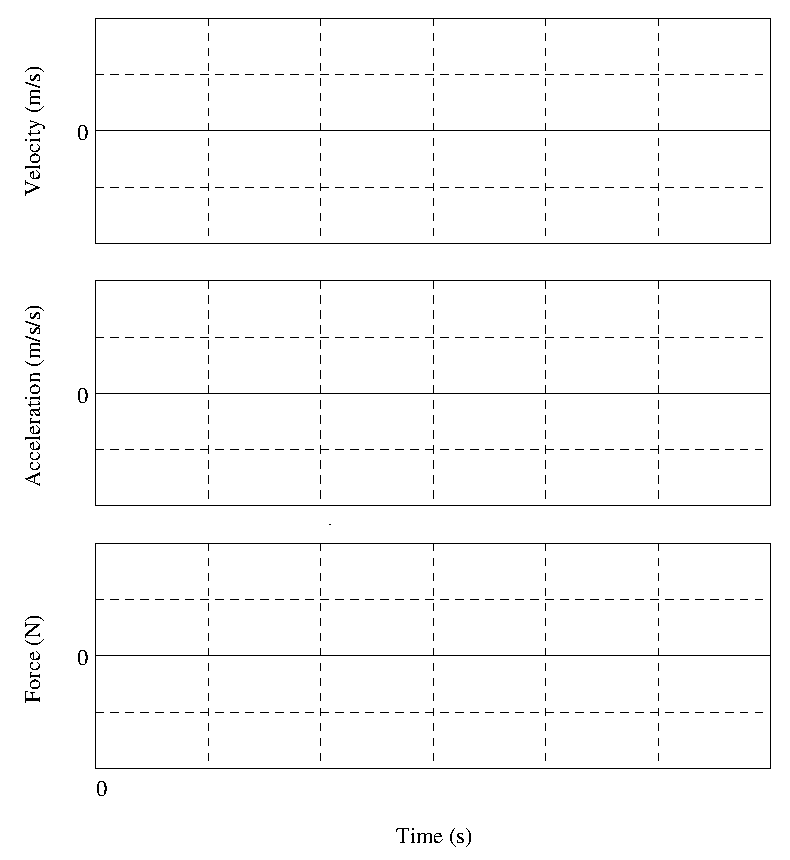
\includegraphics{force2/force2_fig4.eps} \par}
%\vspace{0.3cm}
\begin{lab_groupplot}*{}[lab_grid,
	group style={
		group size=1 by 3,
		xlabels at=edge bottom,
		vertical sep=0.3in,
		},
	width=4.2in,  height=1.4in,
	xlabel=Time (s),
	xmin=0, xmax=12,
	xtick distance = 2, 
	ytick distance = 1, 
	minor tick num=1,
	ytick = {-1,0,1},
	yticklabels = {$-$, 0, $+$},
	]
\nextgroupplot[
	ymin=-1,ymax=1, 
	ylabel={Velocity (m/s)},
	]
\nextgroupplot[
	ymin=-1,ymax=1, 
	ylabel={Acceleration (m/s$^2$)},
	]
\nextgroupplot[
	ymin=-1,ymax=1, 
	ylabel={Force (N)},
	]
\end{lab_groupplot}

(d) Do the graphs agree with your predictions? If not, how do they differ?
\answerspace{20mm}

(e) What happened to the force of the push after you released the cart? Explain.
\answerspace{20mm}

(f) If you give the cart a short push toward the motion detector, how will the
graphs change compared to the ones in this activity for a short push away from
the detector?
\answerspace{20mm}

\pagebreak[2]
\textbf{Comment:} In this activity you have looked at a situation where the
combined force acting on the cart is zero. As you have seen, the velocity of
the cart does not change. The cart either moves with a constant velocity, or
remains at rest. The law, which you have examined in this investigation, describing
the motion when the combined force acting on an object is zero is known as Newton's
First Law.

\textbf{Homework}

In questions 1-4, assume that friction is so small that it can be ignored.

1. The spring scale in the diagram below reads 10.5 N.

\vspace{0.3cm}
{\par\centering 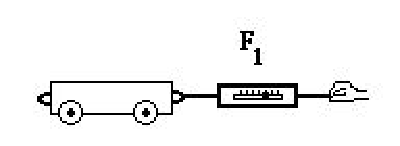
\includegraphics{combining/combining_fig2.eps} \par}
\vspace{0.3cm}

The cart moves toward the right with an acceleration toward the right of 3.50
(m/s)/s. Now two forces are applied to the cart with two different spring scales
as shown below. The spring scale \( F_{1} \) still reads 10.5 N.

\vspace{0.3cm}
{\par\centering 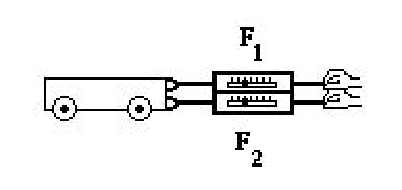
\includegraphics{combining/combining_fig3.eps} \par}
\vspace{0.3cm}

The cart now moves toward the right with an acceleration toward the right of
5.50 (m/s)/s. What does spring scale \( F_{2} \) read? Show your calculations,
and explain.
\answerspace{20mm}

2. Now two forces are applied to the cart with two different spring scales as
shown below. The spring scale \( F_{1} \) still reads 10.5 N.

\vspace{0.3cm}
{\par\centering 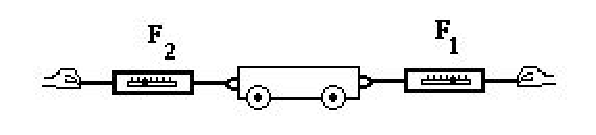
\includegraphics{combining/combining_fig4.eps} \par}
\vspace{0.3cm}

The cart now moves toward the right with an acceleration toward the right of
2.50 (m/s)/s. What does spring scale \( F_{2} \) read?~ Show your calculations,
and explain.
\answerspace{20mm}

\pagebreak[2]
3. Again two forces are applied to the cart with two different spring scales
as shown below. The spring scale \( F_{1} \) still reads 10.5 N.

\vspace{0.3cm}
{\par\centering 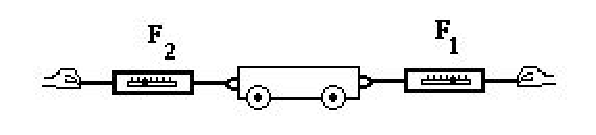
\includegraphics{combining/combining_fig4.eps} \par}
\vspace{0.3cm}

The cart moves with a constant velocity toward the right. What does spring scale
\( F_{2} \) read? Show your calculations, and explain.
\vspace{20mm}

4. Again two forces are applied to the cart with two different spring scales
as shown below. The spring scale \( F_{1} \) still reads 10.5 N.

\vspace{0.3cm}
{\par\centering 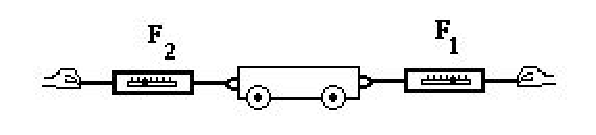
\includegraphics{combining/combining_fig4.eps} \par}
\vspace{0.3cm}

The cart moves toward the left with an acceleration toward the left of 2.50
(m/s)/s. What does spring scale \( F_{2} \) read? Show your calculations, and
explain.

